% !TEX root = paper.tex 
\section{Motivation and Relevance}

Digital wireless communication has become irreplaceable in our modern information technology and society. Communication is done primarily “on the go” using smartphones instead of cable bound landlines. The trusty Ethernet-port is disappearing in modern ultra-slim notebook computers, instead networks are accessed solely via Wi-Fi (IEEE 802.11). Even some household devices such as fridges or even dishwashers can be connected to the internet via Wi-Fi.

Developments like these do no only lead to a world full of exciting new possibilities, but also to a tremendous amount of new potential security risks. Hackers can and do use the ever-growing amount of unsecure or badly secured wireless networks for their own illicit purposes, such as ordering illegal goods or obscuring their access point, or just surfing the internet for free without paying a service provider to access to their infrastructure.  

The reasons to break into a secured wireless network however do not necessarily have to be illegitimate. In fact, the best way to verify a security concept and implementation is to attack it in a controlled and documented manner --- the art of \emph{Penetration testing}.

\section{Testing setup}

To avoid legal issues, a controlled testing setup was constructed for the purpose of this research:

\begin{itemize}

\item{Lenovo Y50-70 \textbf{Laptop} running Kali Linux~\cite{OffSec17} inside a virtual machine}

\item{TP-LINK TL-WN722N \textbf{USB-WiFi antenna}}

\item{TP-LINK TL-WR542G \textbf{wireless router}}

\item{Samsung ATIV-S \textbf{Smartphone} running WP 8.1}

\end{itemize}

A USB antenna was chosen for its extended range and higher transmitting power, compared to the laptops' integrated Wi-Fi antenna. This is especially important when performing attacks where overshadowing another network is the key to successful attack, as shown in Section~\ref{sec:attackuser}.

The operation system \emph{Kali Linux} by \emph{Offensive Security} is a Linux Debian-based system that was initially released in March 2013 as a successor to BackTrack Linux~\cite{OffSecDoc17}. Kali Linux was chosen for its flexibility and vast collection of pre-installed penetration testing software.

Any other devices were already owned and thus chosen because of their availability.

\subsection{Used software}

Kali Linux provides a massive collection of software, engineered for all kinds of use cases. A few specialized programs were used for the purpose of this research:

\begin{itemize}

\item{\textbf{Aircrack-ng suite}~\cite{AirNg17}, capable of using network cards in monitoring mode, capturing packets, decrypting captured traffic and even running active attacks such as deauthentication or packet injection}

\item{\textbf{John the ripper}~\cite{Openwall17}, an advanced password-cracking and hash-breaking tool to use with aircrack-ng}

\item{\textbf{Reaver}~\cite{Reaver17}, a brute-force password cracker}

\item{\textbf{Hashcat}~\cite{Steube17}, an advanced rule-based alternative to John the Ripper}

\item{\textbf{Fluxion}~\cite{Fluxion17}, a social engineering script which is capable of launching evil-twin attacks}

\item{\textbf{Wifiphisher}~\cite{Wifiphisher17}, an advanced alternative to Fluxion}

\end{itemize}

\subsection{Wireless adapter configuration}\label{sec:wificonf}

A Wi-Fi adapter generally can be operated in a multiple distinct modes, \emph{monitor} and \emph{managed} modes. Most household and end-user devices operate in a managed mode, where the networking card acts as a client or access point. In managed mode, the hardware filters the incoming packets before they are forwarded to the operation system. 

Configuring the network card to operate in monitor mode lets the received packets bypass the internal processing unit of the network card and allows the CPU to process the raw packets instead. Also, in monitor mode the network card does not have to be associated to an existing wireless network, making it possible to capture foreign and broken packets or even inject new packets into the network.

Using the above-mentioned aircrack-ng suite, setting the wireless card to monitoring mode can be done by the systems' super user by running

\begin{lstlisting}
airmon start wlan0
\end{lstlisting}

With \lstinline{wlan0} being the desired networking interface. This command will then create an new network interface, \lstinline{wlan0mon}, which exposes the monitoring capability. This can be verified by checking the output of the command \lstinline{iwconfig}.

Not all wireless adapters, drivers and operating systems support using the adapter in monitoring mode. The above configuration has been shown to fulfill all expectations.

\section{Wi-Fi Protected Setup}\label{sec:wps}

Wi-Fi Protected Setup, or \emph{WPS} for short, is a protocol which aims to simplify the process of adding new devices (hereinafter called \emph{Enrollee}) to a wireless network provided by a wireless router (hereinafter called \emph{Registrar}). 

Usually, when using a traditional protocols such as WEP or WPA, the user must enter a password in order to authorize a device. WPS on the other hand allows several quick methods to authorize a device~\cite{WiFi11}, all being based on physical access to the router:

\begin{itemize}

\item{Entering a pre-determined eight digit long \textbf{Personal Indentification Number} (PIN) into the new device. This PIN is often printed on the router itself and is comparable to a regular password. 

However, some models possess a vulnerability where the PIN is derived from the routers' MAC address~\cite{Craig14}, which can be sniffed.}

\item{Via the \textbf{Push Button Configuration} (PBC), where pressing a dedicated hardware button on the router allows new connections for two minutes (See Figure~\ref{fig:wpsbutton}). }

\item{Transferring configuration data using a \textbf{USB Flash Drive} (UFD) from the router to the new device.}

\item{Via \textbf{Near Field Communication} (NFC) where data exchange is achieved by close-range electromagnetic induction.}

\end{itemize}

\begin{figure} %[H]
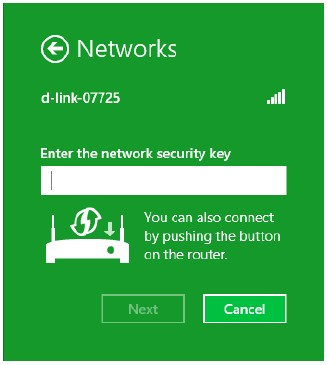
\includegraphics[width=0.3\textwidth]{src/img/DIR-890L-WPS-Button-windows-8c.jpg}
\caption{Connecting to a WPS network in Microsoft Windows 8. From D-Link~\cite{DLink14}}\label{fig:wpsbutton}
\end{figure}

\subsection{Reduced PIN compexity}\label{sec:wpsredpin}

While an eight-digit PIN in itself is already possible to be brute-forced, several flaws in WPS reduce the amount of guesses needed further down~\cite{Ducklin15}. 

Firstly, the last digit of the PIN is a check digit, which can be computed from the other seven. Furthermore, authorization of the enrollee is done in multiple steps~\cite{WiFi06}, in which the enrollee proves possession of the PIN in two stages, one for each half of the PIN (see Table~\ref{tbl:wpskey}).

Because authorization prematurely fails after an invalid first half of the PIN, an attacker only has to guess \(10^4 + 10^3\) times assuming the worst case --- as opposed to the original \(10^8\) times.

\begin{table}[]
\centering
\caption{Composition of a WPS Key}\label{tbl:wpskey}
\begin{tabular}{l|c|c|c|c|c|c|c|l|}
\cline{2-9}
 & \multicolumn{8}{c|}{PIN} \\ \cline{2-9} 
Digit & 1 & 2 & 3 & 4 & 5 & 6 & 7 & \multicolumn{1}{c|}{8} \\ \cline{2-9} 
 & \multicolumn{4}{c|}{First half} & \multicolumn{3}{c|}{Second half} & C \\ \cline{2-9} 
\end{tabular}
\end{table}

\subsection{Flawed random number generator}

Some routers implemented a weak random number generator, which enabled hackers to launch an effective \emph{offline} brute-force attack against captured data from the (failed) WPS PIN handshake~\cite{Bongard14}, called the \emph{Pixiedust} vulnerability.

However, the test device and nearly all devices released within the last few years did not possess this characteristic, so further evaluation was discontinued for the purpose of this research.

\subsection{Attacking with Reaver}\label{sec:reaver}

The \emph{Reaver} password cracker can be used to perform the attack described in Section~\ref{sec:wpsredpin}, after the wireless network adapter has been properly initialized as described in Section~\ref{sec:wificonf}:

\begin{lstlisting}
reaver -i wlan0mon -c 6 -b 00:19:E0:6E:C4:DE -vv
\end{lstlisting}

With \lstinline{6} being the wireless channel in with the router operates, and \lstinline{00:19:E0:6E:C4:DE} the routers' MAC address. 

This information can be found by scanning the network for wireless access points, for example using \lstinline{wash -i wlan0mon} or \lstinline{airodump-ng wlan0mon}. Reaver will then brute-force the WPS PIN, and display it when successful. 

Without special mitigation tactics this process can take up to a few hours, or just a few minutes when a \emph{Pixiedust} vulnerability is detected.

\section{Wired Equivalent Privacy}

Wired Equivalent Privacy, or \emph{WEP} for short, is a deprecated jet still used Wi-Fi authorization and encryption protocol.

Data is encrypted by XOR-ing it with a pseudorandom stream of data (see Figure~\ref{fig:wepmech}), which is generated using the RC4-Algorithm~\cite{WiFi16}.

The RC4 random number generator is initialized with the concatenation of an 24-bit \emph{Initialization Vector} (IV) and the actual hexadecimal password. The width of the seed can range from 64 to 256 bits in some implementations.

\begin{figure}

\includegraphics[width=0.4\textwidth]{src/img/Wep-crypt-alt.png}
\caption{Basic WEP encryption mechanism. From Wikipedia, the free encyclopedia~\cite{BHL07}}\label{fig:wepmech}
\end{figure}

\subsection{Related-Key vulnerability}

The RC4 random number generator is vulnerable to the \emph{Fluhrer, Mantin and Shamir attack}~\cite{FMS01}.

Exploiting this flaw using certain generated IVs, an attacker can --- knowing the first byte of the key stream and the first n bytes of a key --- derive the next byte of this key.

To receive enough (a few thousand) IVs, an attacker has to choose a rather busy network and/or collect packets for a long period of time.

The recoded IVs can then be used to deduce the original key und consequently the password.

\subsection{Increasing the amount of IVs}

The router can be provoked to send a massive amounts of packages by spamming it with ARP requests, to which the router is obliged to answer.

Newer models counteract this by strategically stalling replies when an ARP flooding is detected.

\subsection{Attacking with Aircrack}\label{sec:wepcrack}

Using the \emph{Aircrack} software suite, it is possible to break into a WEP secured network as discussed above. After the wireless adapter has been properly initialized (see Section~\ref{sec:wificonf}), an a taget router has been identified, a background process record all received packets into a log file:

\begin{lstlisting}
airodump-ng -c 6 --essid enigma -w logfile_name wlan0mon
\end{lstlisting}

Here, the \lstinline{c} and \lstinline{essid} flags specify the wireless channel and access point SSID, similar to the attack in Section~\ref{sec:reaver}.

In parallel, the attacker prepares an \emph{ARP-replay attack} by first performing a \emph{fake authentification} via the \emph{WEP open system authentification}, where any device can pair with the router without actually being allowed to access the internet~\cite{WiFi16}:

\begin{lstlisting}
aireplay-ng -1 0 -e enigma -a 00:19:E0:6E:C4:DE -h 18:D6:C7:0C:76:B8 wlan0mon
\end{lstlisting}

The \lstinline{e} flag to specify the SSID is optional when same is not hidden.

After successfully associating the attackers' MAC address (specified via the \lstinline{h} flag), the attacker waits for a legitimate ARP packet to be sent, and then sends massive amounts of copies to the router (often with rates of several hundred packets per second):

\begin{lstlisting}
aireplay-ng -3 -b 00:19:E0:6E:C4:DE -h 18:D6:C7:0C:76:B8 wlan0mon
\end{lstlisting}

This causes the router to retransmit every ARP response with a new IV --- dramatically reducing the time needed for sufficient package capture down to a few minutes.

Using the captured package data, the attacker can then deduce the original password offline:

\begin{lstlisting}
aircrack-ng logfile_name.cap
\end{lstlisting}

This process is very fast and requires usually a few ten thousand different IVs.

\section{Wi-Fi Protected Access}

Faced with the serious security vulnerabilities in WEP, the Wi-Fi Alliance came up with \emph{Wi-Fi Protected Access} (WPA) in 2003 and its successor \emph{WPA2} in 2004.

The most commonly used protocol, WPA2-PSK, uses a \emph{pre-shared key} (PSK) to validate potential new devices. This is done by entering a user determined password.

As of today (July 2017), there a no publicly known effective technical attacks against WPA2-PSK other than determining the key by brute force.

\subsection{Four-way handshake}\label{sec:wpa2handshake}

WPA2-PSK uses a four-way handshake (see Figure~\ref{fig:wpa2fway}) to mutually verify knowledge of the password without actually disclosing it to each other~\cite{WiFi16}. Note that this technique is similar to WPS PIN-based authorization (see Section~\ref{sec:wps}), done in a more secure manner.

Because the actual password is only used during the authorization, an attacker has to record a handshake and then try to crack it.

\subsection{Deauthentication attack}\label{sec:deauth}

When sending fake deauthentication packets to the router and simultaneously spoofing their own MAC address (using the one of their victim), the wireless router logs off the victim.

The attacker then just has to wait for he victim to reconnect (which often happen automatically) and record the handshake.

\begin{figure}

\includegraphics[width=0.4\textwidth]{src/img/4-way-handshake.png}
\caption{The four-way handshake of WPA2-PSK. From Wikipedia, the free encyclopedia~\cite{Mikm07}}\label{fig:wpa2fway}
\end{figure}

\subsection{Attacking with brute force}\label{sec:wpa2brute}

To perform the attack described above, an attacker first logs all packets using a background process as demonstrated in Section~\ref{sec:wepcrack} after having the wireless adapter properly initialized (see Section~\ref{sec:wificonf}).

Meanwhile the \lstinline{aireplay} software is used to send a fake deauthentication message:

\begin{lstlisting}
aireplay-ng -0 1 -a 00:19:E0:6E:C4:DE -c C4:88:E5:90:98:84 wlan0mon
\end{lstlisting}

Here the \lstinline{a} flag specifies the MAC address of the wireless router, while the \lstinline{c} flag specifies the victims' MAC address.

The background packet logging process will then signal the capture of a WPA2 handshake.

Using a list of commonly used passwords, a so-called \emph{rainbow table}, the attacker can then start to try out keys.

\begin{lstlisting}
aircrack-ng -w wordlist.txt -b 00:19:E0:6E:C4:DE logfile_name.cap
\end{lstlisting}

The success and duration of this method strongly depend on the quality of the chosen password list.

However, it is possible to use auxiliary software to generate commonly used passwords. Using the program \emph{Jack the ripper}, the attacker can automate the process of password guessing:

\begin{lstlisting}
john --stdout --incremental:LowerNum | aircrack-ng -w -- -b 00:19:E0:6E:C4:DE logfile_name.cap
\end{lstlisting}

In this example, the generator incrementally creates alphanumerical passwords and then redirects its output to the password testing utility. On the virtualized testing system, it was possible to test about 3000 keys on average per second.

Using this estimate, testing all possible simple 10-letter alphanumeric keys would take about \(8.9\) \emph{million} years (assuming 26 letters, two cases and ten digits):

\begin{displaymath}
\frac{(26 * 2 + 10)^{10}}{3000\frac{k}{s}}\approx2.8*10^{14} s
\end{displaymath}

This shows that the key to fast password recovery is intelligent guessing. Software like \emph{Hashcat}~\cite{Steube17} for example is able to test passwords based on complex rules and user-supplied keywords.

Especially when combined with previously obtained personal information about the victim, this technique reduces the password guessing time dramatically.

\section{Social engineering}\label{sec:attackuser}

When attempting to break into WPA2-PSK networks, even the best password guessing algorithm and an extreme fast and parallel computing platform are no match to a long and complex (or even random) password (see Section~\ref{sec:wpa2brute}).

Humans users are however, compared to computer-based authorization algorithms, rather gullible. 

\emph{Social engineering} is the act of acquiring protected information not by purely technical hacking, but by social means like tricking inexperienced users into revealing passwords, or finding sticky notes in the trash.

\subsection{Evil twin phishing attack}\label{sec:eviltwin}

A commonly used and rather effective method to acquire a WPA2 password works by tricking a user into revealing it to the attacker.

This is done by suppressing and posing as the original wireless router as shown in Figure~\ref{fig:eviltwin}, called an \emph{evil twin attack}.

\begin{figure}
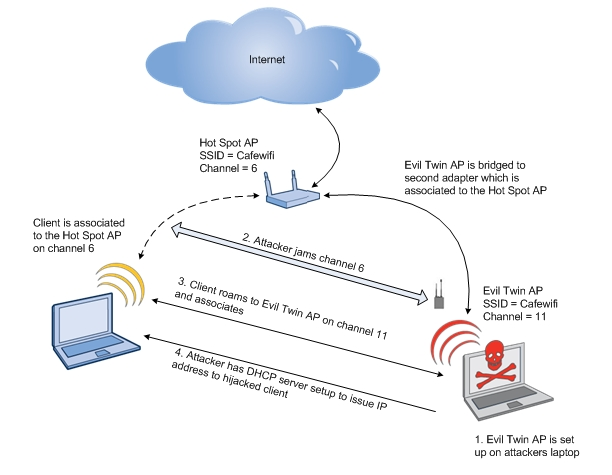
\includegraphics[width=0.5\textwidth]{src/img/38_1.jpg}
\caption{Evil twin attack. From Hackinsight~\cite{Hackinsight14}}\label{fig:eviltwin}
\end{figure}

After successfully having lured the victim into trusting the fake access point, the attacker then presents the victim with a website where the WPA key is to be entered, allegedly to re-access the network.

On the technical side this is done in several steps:

\begin{enumerate}

\item{Scanning for access points and potential victims}

\item{Setting up a virtual access point on the attackers' system using a free wireless channel}

\item{Deauthenticating the victim (see Section~\ref{sec:deauth})}

\item{Jamming the old wireless channel by continuing to deauthenticatenew clients, threfore forcing the victim to connect to the attackers' access point}

\item{Modifying DNS lookups by running a custom DNS server to redirect the victim to a login prompt}

\item{Providing a login prompt via HTTP}

\item{Capturing the entered passsword}

\item{\textbf{Optional:} Validating the entered password by testing it against a previously captured WPA2 four-way handshake (see Section~\ref{sec:wpa2handshake})}

\item{Shutting down all fake systems}

\end{enumerate}

Though it is possible to do all these steps by hand, several software utilities were developed to automate this process, two of them being \emph{Fluxion}~\cite{Fluxion17} and \emph{Wifiphisher}~\cite{Wifiphisher17}, which both provide a command-line based interface.

Crucial to the success of this phishing attack is the credibility of the displayed password prompt and the good faith of the victim. 

If the wireless routers' model is known, one possible way to feign credibility is to fake a firmware update legitimation prompt. In a hotel or similar institution network, faking the regular login page can also yield the wanted results.

\section{Conclusion}

Wrapping up, there really is no way to provide 100\% unbreakable wireless network security. However, it is possible to make it extraordinarily hard for an attacker to breach a network. 

This can be done on the technical side by:

\begin{itemize}

\item{Disabeling deprecated protocols like WEP and WPS and upgrading to WPA2-PSK}

\item{Using a per-user authentification system}

\item{Picking long and complex pre-shared keys and passwords}

\item{Keeping the wireless routers' firmware up-to-date}

\item{Restricting physical access to the wireless router}

\end{itemize}

And on the social side by:

\begin{itemize}

\item{Implementing strict password policies}

\item{Educating users about phishing and social engineering attacks}

\item{Demonstrating attacks to sensitize users to tell-tale signs of such attacks}

\end{itemize}